\chapter{Thực nghiệm Sư phạm}

\section{Mục tiêu thực nghiệm}\begin{itemize}
	\item Tìm hiểu khả năng ứng dụng AI vào đánh giá năng lực của học sinh.
	\item Phân tích sự chính xác của kết quả kiểm tra thích ứng so với điểm trung bình môn Toán của học sinh, từ đó nhận xét về tính khả quan của Kant bot trong đánh giá năng lực học sinh.
	\item Cải tiến và hoàn thiện Kant bot.
\end{itemize}

\section{Đối tượng và tiến trình thực nghiệm}
\subsection{Đối tượng thực nghiệm}
	38 học sinh lớp 11, 12 thuộc các trường THPT Châu Văn Liêm, Lý Tự Trọng và Thực hành Sư phạm.

\subsection{Tiến trình thực nghiệm}
\begin{enumerate}[label=\textbf{Giai đoạn \arabic*.},align=left,left=0cm..0cm,itemindent=*]
	\item Gửi đường link truy cập cho học sinh làm thực nghiệm phần Tổ hợp – Xác suất với sự đánh giá tự động của Kant bot.\par
	\item Phân tích quá trình đánh giá của Kant đối với một số học sinh.
	\item Tổng hợp và phân tích kết quả đánh giá của học sinh.
\end{enumerate}

\section{Nội dung thực nghiệm}
Quá trình thực nghiệm chính được thực hiện hoàn toàn trực tuyến với Kant bot, thông qua nền tảng Facebook Messenger.\par
Trong phần này, người dùng cần phải thực hiện tối đa 10 câu hỏi trắc nghiệm cho một chủ đề – với câu hỏi được đưa ra dựa trên dữ liệu trả lời những câu hỏi trước – để đạt tới mức kỳ vọng ổn định nhất (kỳ vọng dưới $1$). Sau đó Kant sẽ đưa ra kết quả đánh giá năng lực. Hình \ref{fig:fig-c4-chatbot-demo} minh họa quá trình thực nghiệm đánh giá với Kant.
\begin{figure}[htb!]\centering
	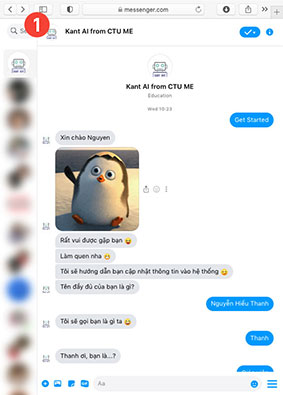
\includegraphics[width=7cm]{kant-ux/chat-1}
	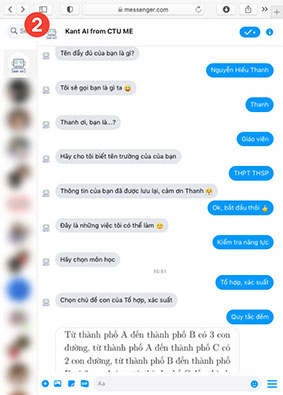
\includegraphics[width=7cm]{kant-ux/chat-2}
	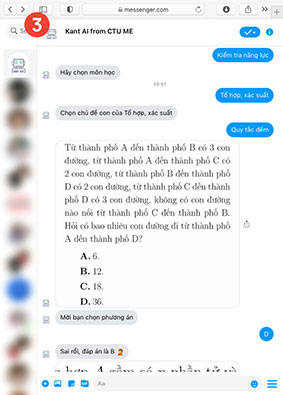
\includegraphics[width=7cm]{kant-ux/chat-3}
	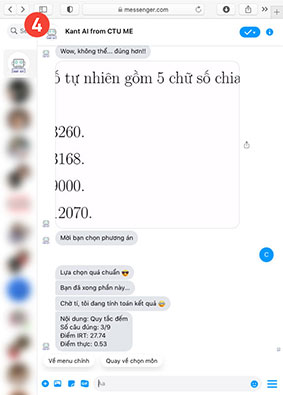
\includegraphics[width=7cm]{kant-ux/chat-4}
	\caption{Minh họa quá trình thực nghiệm với Kant}
	\label{fig:fig-c4-chatbot-demo}
\end{figure}\par

\section{Kết quả thực nghiệm}

Có 38 học sinh hoàn thành phần kiểm tra năng lực chương Tổ hợp, xác suất. Kết quả đánh giá năng lực bằng Kant bot được tổng hợp ở bảng \ref{tab:tab-s4-result}, danh sách được sắp xếp và đặt mã số theo \textit{Sai số} giảm dần.

\begin{longtable}{ScSlScScScSc}
	\caption{Kết quả thực nghiệm đánh giá bằng Kant bot}\label{tab:tab-s4-result}\\
	\textbf{TT} & \multicolumn{1}{Sc}{\textbf{Trường THPT}} & \textbf{Lớp} & \textbf{KQ đánh giá} & \textbf{ĐTB Toán} & \textbf{Sai số} \\ \hline\endfirsthead

	\textbf{TT} & \multicolumn{1}{Sc}{\textbf{Trường THPT}} & \textbf{Lớp} & \textbf{KQ đánh giá} & \textbf{ĐTB Toán} & \textbf{Sai số} \\ \hline\endhead\hline\endfoot

	S01 & Thực hành Sư phạm & 11 & $8.5$ & $8.5$ & $0.0$ \\
	S02 & Thực hành Sư phạm & 11 & $9.6$ & $9.5$ & $0.1$ \\
	S03 & Châu Văn Liêm     & 12 & $8.0$ & $8.1$ & $0.1$ \\
	S04 & Thực hành Sư phạm & 11 & $8.8$ & $8.7$ & $0.1$ \\
	S05 & Thực hành Sư phạm & 12 & $9.4$ & $9.6$ & $0.2$ \\
	S06 & Thực hành Sư phạm & 11 & $9.4$ & $9.6$ & $0.2$ \\
	S07 & Thực hành Sư phạm & 11 & $7.8$ & $8.0$ & $0.2$ \\
	S08 & Lý Tự Trọng       & 12 & $9.5$ & $9.1$ & $0.4$ \\
	S09 & Thực hành Sư phạm & 11 & $8.9$ & $8.5$ & $0.4$ \\
	S10 & Thực hành Sư phạm & 11 & $6.1$ & $6.5$ & $0.4$ \\
	S11 & Thực hành Sư phạm & 11 & $9.1$ & $9.6$ & $0.5$ \\
	S12 & Lý Tự Trọng       & 12 & $8.9$ & $9.4$ & $0.5$ \\
	S13 & Thực hành Sư phạm & 11 & $9.5$ & $9.0$ & $0.5$ \\
	S14 & Châu Văn Liêm     & 12 & $6.9$ & $7.4$ & $0.5$ \\
	S15 & Châu Văn Liêm     & 12 & $8.7$ & $8.0$ & $0.7$ \\
	S16 & Thực hành Sư phạm & 11 & $9.8$ & $9.1$ & $0.7$ \\
	S17 & Thực hành Sư phạm & 11 & $8.8$ & $8.0$ & $0.8$ \\
	S18 & Thực hành Sư phạm & 11 & $7.9$ & $9.0$ & $1.1$ \\
	S19 & Thực hành Sư phạm & 11 & $6.9$ & $8.0$ & $1.1$ \\
	S20 & Lý Tự Trọng       & 12 & $7.2$ & $8.5$ & $1.3$ \\
	S21 & Thực hành Sư phạm & 11 & $9.8$ & $8.5$ & $1.3$ \\
	S22 & Châu Văn Liêm     & 12 & $7.0$ & $8.4$ & $1.4$ \\
	S23 & Thực hành Sư phạm & 11 & $6.7$ & $8.2$ & $1.5$ \\
	S24 & Thực hành Sư phạm & 11 & $6.9$ & $8.5$ & $1.6$ \\
	S25 & Thực hành Sư phạm & 11 & $6.9$ & $8.5$ & $1.6$ \\
	S26 & Thực hành Sư phạm & 11 & $5.0$ & $6.7$ & $1.7$ \\
	S27 & Thực hành Sư phạm & 11 & $5.3$ & $7.2$ & $1.9$ \\
	S28 & Châu Văn Liêm     & 12 & $6.5$ & $8.6$ & $2.1$ \\
	S29 & Thực hành Sư phạm & 12 & $5.0$ & $7.1$ & $2.1$ \\
	S30 & Thực hành Sư phạm & 11 & $2.9$ & $5.0$ & $2.1$ \\
	S31 & Thực hành Sư phạm & 11 & $6.9$ & $9.1$ & $2.2$ \\
	S32 & Lý Tự Trọng       & 11 & $6.9$ & $9.1$ & $2.2$ \\
	S33 & Thực hành Sư phạm & 11 & $6.9$ & $9.2$ & $2.3$ \\
	S34 & Lý Tự Trọng       & 12 & $6.2$ & $8.5$ & $2.3$ \\
	S35 & Thực hành Sư phạm & 11 & $7.0$ & $9.4$ & $2.4$ \\
	S36 & Thực hành Sư phạm & 11 & $6.0$ & $8.6$ & $2.6$ \\
	S37 & Thực hành Sư phạm & 11 & $6.2$ & $9.0$ & $2.8$ \\
	S38 & Châu Văn Liêm     & 12 & $6.6$ & $9.5$ & $2.9$ \\
\end{longtable}\par

\subsection{Phân tích phân phối kết quả}

Các kết quả đánh giá được thống kê lại theo các mốc: \begin{itemize}
	\item \textit{Giỏi}: Từ $8.0$ trở lên.
	\item \textit{Khá}: Từ $6.5$ tới dưới $7.9$.
	\item \textit{Trung bình}: Từ $5.0$ tới dưới $6.4$.
	\item \textit{Yếu}: Từ $3.5$ tới dưới $4.9$.
	\item \textit{Kém}: Dưới $3.5$.
\end{itemize}\par

\begin{longtable}{SlScScScSc}
	\multirow{2}{*}{\bfseries Nhóm} & \multicolumn{2}{Sc}{\bfseries KQ đánh giá} & \multicolumn{2}{Sc}{\bfseries ĐTB Toán}\\\cline{2-5}
	& Tần số & Tỉ lệ & Tần số & Tỉ lệ \\\hline\endhead\hline\endfoot
	Giỏi       & $15$ & $39.5\%$ & $32$ & $84.2\%$ \\
	Khá        & $15$ & $39.5\%$ &  $5$ & $13.2\%$ \\
	Trung bình &  $7$ & $18.4\%$ &  $1$ &  $2.6\%$ \\
	Yếu        &  $-$ & $-$ & $-$ & $-$ \\
	Kém        &  $1$ &  $2.6\%$ &  $-$ & $-$ \\
\end{longtable}\par

Đề tài tiến hành kiểm định tính chính xác của kết quả đánh giá, tức là kiểm định tính độc lập giữa hai biến \textit{KQ đánh giá} và \textit{ĐTB Toán}. Ở đây, mỗi học sinh được phân loại theo hai đặc tính là \textit{KQ đánh giá} (đặt là biến $X$) và \textit{ĐTB Toán} (đặt là biến $Y$). Có 4 giá trị cho biến $X$ (giỏi, khá, trung bình, kém) và 3 giá trị cho $Y$ (giỏi, khá, trung bình) nên $$P_{ij}=P(X=x_i,Y=y_j),~i=\overline{1,4},~j=\overline{1,3}.$$
là xác suất chọn được học sinh mạng đặc tính $X$ là $x_i$ và đặc tính $Y$ là $y_j$. Gọi
$$p_i=P(X=x_i)=\sum_{j=1}^{3}P_{ij},~i=\overline{1,4},$$
$$q_j=P(Y=y_j)=\sum_{i=1}^{4}P_{ij},~j=\overline{1,3}.$$
Trong đó $p_i$ là xác suất chọn được học sinh có $X=x_i$, $q_j$ là xác suất chọn được học sinh có $Y=y_j$.\par
Phát biểu giả thuyết:
\begin{align*}
	H_0:~&P_{ij}=p_iq_j,~\forall i=\overline{1,4},~j=\overline{1,3}.\\
	H_1:~&\exists (i,j) | P_{ij}\neq p_iq_j.
\end{align*}\par

Từ kết quả thực nghiệm đánh giá (bảng \ref{tab:tab-s4-result}), thu được bảng kết quả như sau:
\begin{longtable}{ScSlScScScSc}
	& & \multicolumn{3}{Sc}{\bfseries ĐTB Toán} & \multirow{2}{*}{\bfseries Tổng}\\\cline{3-5}
	& & Giỏi & Khá & Trung bình &\\\hline\endhead\hline\endfoot
	\multirow{4}{*}{\textbf{KQ đánh giá}}
	& Giỏi       & 15 & – & – & 15\\
	& Khá        & 14 & 1 & – & 15\\
	& Trung bình & 3  & 4 & – & 7 \\
	& Kém        & 0  & 0 & 1 & 1 \\\hline
	\multicolumn{2}{Sc}{\textbf{Tổng}} & 32 & 5 & 1 & 38
\end{longtable}\par

Kết quả kiếm định độc lập bằng phần mềm SPSS được cho trong bảng \ref{tab:tab-s4-chi-square} dưới đây:
\begin{longtable}{SlSrScSc}
	\caption{Kết quả kiểm định ($\chi^2$) \textit{KQ đánh giá} với \textit{ĐTB Toán}}\label{tab:tab-s4-chi-square}\\
	& \multicolumn{1}{Sc}{\bfseries Value} & \textbf{df} & \textbf{A. Sign. (2-sided)}\\\hline\endfirsthead

	& \multicolumn{1}{Sc}{\bfseries Value} & \textbf{df} & \textbf{A. Sign. (2-sided)}\\\hline\endhead\hline\endfoot
	\textbf{Pearson Chi-Square} & $52.734$ & $6$ & $<0.001$\\
	\textbf{Likelihood Ratio} & $21.646$ & $6$ & $0.001$\\
	\textbf{N of Valid Cases} & 38 & &\\
\end{longtable}
Kết quả $p\mathrm{-value}=0.001<5\%$ nên có thể bác bỏ giả thuyết $H_0$ tại mức ý nghĩa $5\%$ và kết luận rằng \textit{KQ đánh giá} phụ thuộc vào \textit{ĐTB Toán}. Hơn nữa, điều này khẳng định việc đánh giá năng lực học sinh thông qua Kant bot là hoàn toàn khả quan.\par

Tiếp đến, đề tài tiến hành ước lượng sai số trong đánh giá, kết quả được cho ở bảng \ref{tab:tab-s4-explore}.
\begin{longtable}{SlSlScSc}
	\caption{Kết quả ước lượng \textit{Sai số} đánh giá}\label{tab:tab-s4-explore}\\
	& & \textbf{Statistic} & \textbf{Std. Error} \\\hline\endfirsthead

	& & \textbf{Statistic} & \textbf{Std. Error} \\\hline\endhead\hline\endfoot

	\multicolumn{2}{Sl}{Mean} & $1.232$ & $0.1449$\\
	\multirow{2}{*}{\begin{minipage}{3.5cm}Confidence Interval for Mean\end{minipage}}
	& Lower Bound & $0.987$&\\
	& Upper Bound & $1.476$  &\\
	\multicolumn{2}{Sl}{5\% Trimmed Mean}    & $1.207$  &\\
	\multicolumn{2}{Sl}{Median}              & $1.2$    &\\
	\multicolumn{2}{Sl}{Variance}            & $0.797$  &\\
	\multicolumn{2}{Sl}{Std. Deviation}      & $0.8929$ &\\
	\multicolumn{2}{Sl}{Minimun}             & $0.0$    &\\
	\multicolumn{2}{Sl}{Maximum}             & $2.9$    &\\
	\multicolumn{2}{Sl}{Range}               & $2.9$    &\\
	\multicolumn{2}{Sl}{Interquartile Range} & $1.7$    &\\
	\multicolumn{2}{Sl}{Skewness}            & $0.249$  & $0.383$\\
	\multicolumn{2}{Sl}{Kurtosis}            & $-1.313$ & $0.750$\\
\end{longtable}\par

Với độ tin cậy $90\%$, \textit{Sai số} đánh giá so với \textit{ĐTB Toán} của học sinh được ước lượng nằm trong đoạn $[0.987;1.476]$ nhìn chung khá lớn, tuy nhiên đây chỉ là bài kiểm tra năng lực của một chủ đề (phần Tổ hợp, xác suất), do đó hoàn toàn có thể chấp nhận được. Bên cạnh đó, \textit{độ lệch chuẩn} (standard deviation) của \textit{Sai số} là $0.8929<1$ – hoàn toàn tương ứng với điều kiện dừng của thuật toán (dừng kiểm tra khi kỳ vọng nhỏ hơn $1$).\par

\subsection{Phân tích quá trình đánh giá một số học sinh}

Đề tài chọn phân tích 03 kết quả ngẫu nhiên của các học sinh có \textit{Sai số} lần lượt là $0$ (giá trị nhỏ nhất – minimum), $2.9$ (giá trị lớn nhất – maximum) và $0.5$ (yếu vị – mode), cụ thể là S01, S38 và S12.\par

